\chapter{ABR Module for ns-3}
\label{chap:abrmodule}

This chapter will introduce a new module for \textit{ns-3} for ABR streaming simulation.
The \autoref{sec:abrobj} will set the objective and the scope of the design. 
The \autoref{sec:abrarch} will present the architecture of the module.
The \autoref{sec:abrmodels} will go over the models the module is composed of.
Finally, the \autoref{sec:abralgo} will explain the adaptation algorithms implemented in this module.


\section{Design Objectives}
\label{sec:abrobj}
The main objective of this chapter is to design and implement a \textit{ns-3} module able 
to simulate the behavior of video streaming devices in mobile network scenarios. To build 
a framework capable of testing new adaptation algorithms and be possible to extract metrics 
to measure quality of services and quality of experience.

\section{Architecture}
\label{sec:abrarch}

The ABR module provides:
\begin{itemize}[noitemsep,topsep=0pt]
  \item \texttt{\textbf{AbrClient}}. This class mimics a video streaming application. It has an instance 
  of \texttt{AbrAlgorithm}, which is responsible of 
  deciding which quality of media content to download from the \texttt{AbrServer}.
  It is an implementation of \texttt{ns3::Application}.
  \item \texttt{\textbf{AbrServer}}. This class simulates a video streaming HTTP server. It receives
  requests from clients and sends the multimedia segments requested. It is an implementation of 
  \texttt{ns3::Application}.
  \item \texttt{\textbf{AbrVariables}}. This class is used for storing common variables between the clients
  and the servers. It contains the definition of Segment, Representation, AbrTask, etc.
  \item \texttt{\textbf{AbrHelper}}. This is a Helper class for the ABR module. It is the responsible 
  for managing the instances of the ABR clients and servers. In addition, \texttt{AbrHelper} can be
  used for extracting QoS and QoE metrics.
  \item \texttt{\textbf{AbrAlgorithm}}. This is a base class to be implemented with different 
  adaptation algorithms.
  \item \texttt{\textbf{HLSjs}}. This is an implementation of \texttt{AbrAlgorithm} based on \cite{hls3}.
  \item \texttt{\textbf{DASHjs}}. This is an implementation of \texttt{AbrAlgorithm} based on \cite{dash3}. 
  It also contains the implementation of the buffer based BOLA algorithm.
  \item \texttt{\textbf{abr-example.cc}}. An basic example script with two nodes linked with a
  \texttt{PointToPoint} connection and a unstable connection.
\end{itemize}

\begin{figure}[]
  \centering
  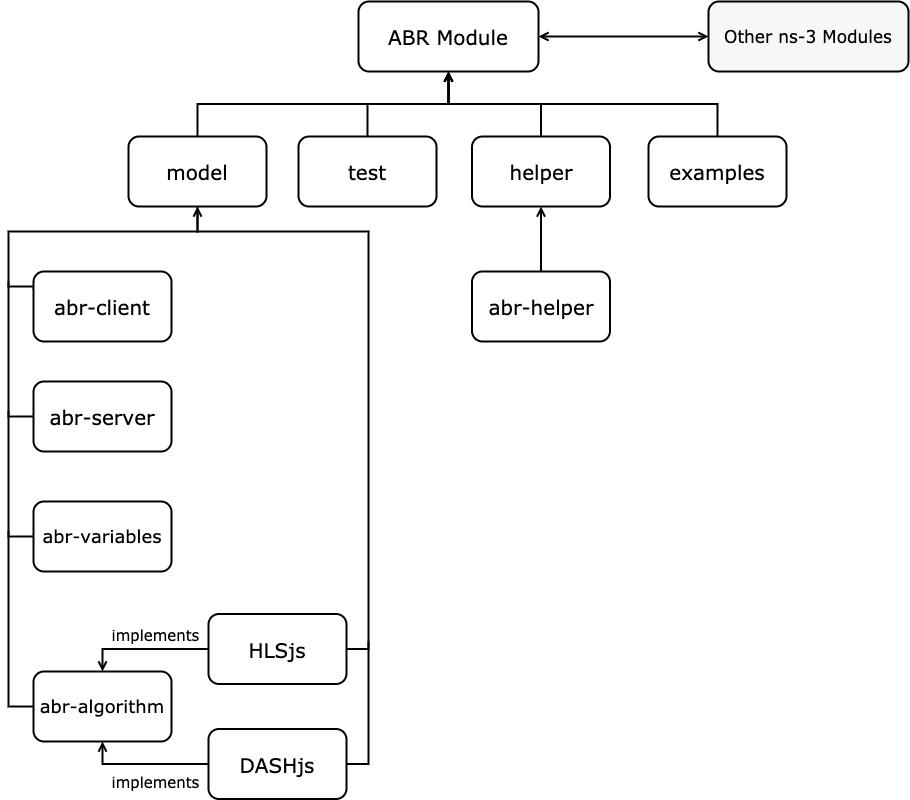
\includegraphics[width=\textwidth]{img/abr.png}
  \caption{ABR Module architecture.}
  \label{fig:abrarch}
\end{figure}

The \autoref{fig:abrarch} shows the architecture of the ABR module. Although this module 
was designed to be used in mobile environments, it can be used with any other \texttt{Application} 
class in \textit{ns-3}, meaning that the ABR clients and servers can be installed in any \texttt{Node}
and work with other \textit{ns-3} modules and models.


\section{Models}
\label{sec:abrmodels}
This section will go through all the models, classes and helpers in the ABR module and how they work 
together.


\subsection{AbrClient}
The \texttt{AbrClient} is an implementation of \texttt{ns3::Application}. This class 
uses an implementation of \texttt{AbrAlgorithm} to create HTTP-like requests to the 
\texttt{AbrServer} and mimics the playing of the media content.

The \texttt{AbrClient} is created with the \texttt{AbrHelper} and the server address and port as
parameters.
Then the client application needs to be installed
on the client nodes. When the simulation starts, the function \texttt{StartApplication} is called
and the simulator is scheduled to call \texttt{HandlePlay} function to simulate video watching.
The client will create a new socket, in this case a TCP socket, to connect with the server.
The socket is set will various callback functions:
\begin{itemize}[noitemsep,topsep=0pt]
  \item \texttt{ConnectionSucceded}. is called if the connection succeeded. Then it calls
  the \texttt{CheckAlgorithm} function.
  \item \texttt{ConnectionFailed}. is called if the connection failed. This should not 
  happen if the simulation script is correctly written.
  \item \texttt{HandleRead}. is called when new packets are received. It stores the segments 
  to the segment buffer, and checks the adaptation algorithms after one entire segment is downloaded.
\end{itemize}

The \texttt{CheckAlgorithm} method asks the \texttt{AbrAlgorithm} and returns
one or more \texttt{AbrTasks}. The client will call the scheduled 
functions depending on the designated task and delay.

\begin{figure}[]
  \centering
  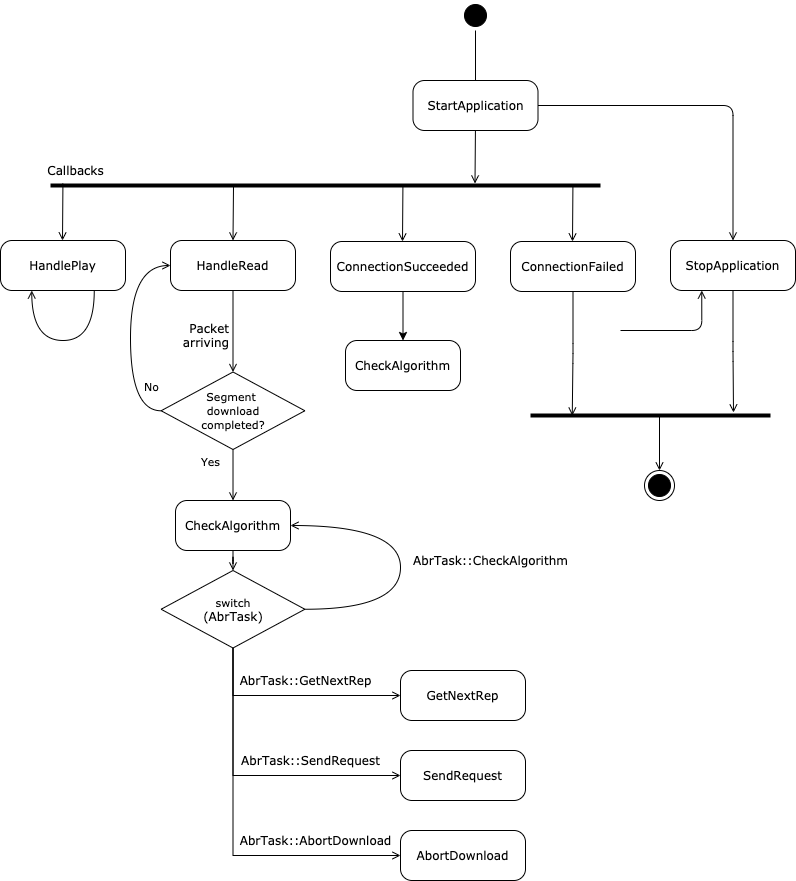
\includegraphics[width=\textwidth]{img/abrclient.png}
  \caption{ABR Client.}
  \label{fig:abrclient}
\end{figure}

\subsection{AbrServer}

The \texttt{AbrServer} is an implementation of \texttt{ns3::Application}. This class 
receives HTTP-like requests from the \texttt{AbrClient} and sends the requested segment.

The request is in the format:

\begin{itemize}[noitemsep, topsep=0pt]
  \centering
  \item[] \texttt{\textbf{GET qualityIndex numberOfSegments startSegment}}
\end{itemize}

For example, "\texttt{GET 4 1 3}" means "GET 1 segment of quality index 4 starting from the 
${3^{rd}}$ segment".


\begin{figure}[h]
  \centering
  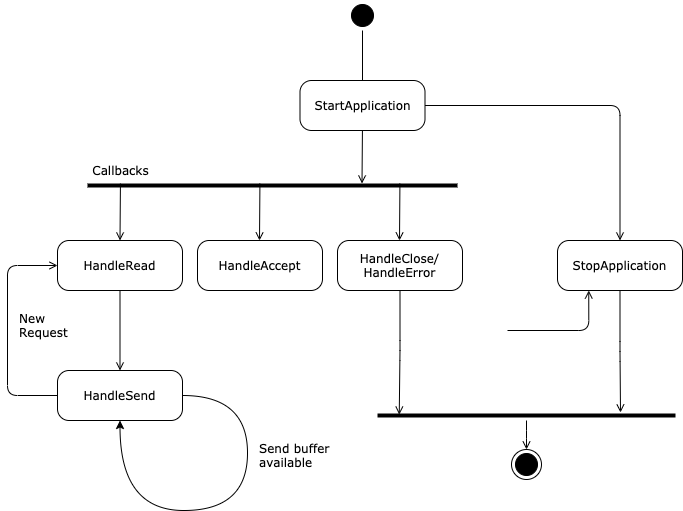
\includegraphics[width=0.95\textwidth]{img/abrserver.png}
  \caption{ABR Server.}
  \label{fig:abrserver}
\end{figure}


The \texttt{AbrServer} is created with the \texttt{AbrHelper} and the listening port as the 
parameter. Then the
server application needs to be installed on the server node. When the simulation starts, the 
function \texttt{StartApplication} is called. The server will create a socket, binds it and starts
to listen.
The socket is set will callback functions. When the sockets are connected, the server 
will schedule new callbacks to handle reading requests and sending data.


\subsection{AbrVariables}

The \texttt{AbrVariables} class contains variables and functions used by the
\texttt{AbrClient} and \texttt{AbrServer}, including the definition of 
a set of essential data structures. These data structures are:

\begin{itemize}[noitemsep, topsep=0pt]
  \item \texttt{\textbf{Segment}}. It is an abstraction of a media segment. A \texttt{Segment} 
  has a size (in bytes), a start time and a duration.
  \item \texttt{\textbf{Representation}}. Describes a certain version of a encoded media. A \texttt{Representation}
  include the resolution, the frames per second and the encoding bitrate.
  \item \texttt{\textbf{SegmentInfo}}. This is a aditional data structure for \texttt{Segment}. A \texttt{SegmentInfo} contains 
  information about download start/finish time, playback start/finish time, the bandwidth estimation
  used to download that segment and the quality index of the segment.
  \item \texttt{\textbf{PlayerStates}}. This class keeps track on the player status.
  \item \texttt{\textbf{AbrTask}}. An \texttt{AbrTask} is a used to schedule tasks for \texttt{AbrClients}.
\end{itemize}

\texttt{AbrVariables} has these variables:
\begin{itemize}[noitemsep, topsep=0pt]
  \item \texttt{\textbf{m\_segments}}. It is a two-dimentional vector containing all the segments 
  for the simulation. Each row has de the same quality and the higher the row index, the higher the
  quality. The segments are ordered in time in the columns.
  \item \texttt{\textbf{m\_representations}}. It is a vector containing all the \texttt{Representations}.
  The row index also means the quality level.
  \item \texttt{\textbf{m\_segmentDuration}}. The duration of the segment in milliseconds. By default, it is ${2000ms}$.
\end{itemize}

Before the simulation starts, the \texttt{AbrVariables} class initializes the
variables. Starting with the representations, there are a predefined set of \texttt{Representations}
by default, but they can be changed in the source file. 
Continuing with the segments, their sizes are calculated based on the resolution,
framerate and the encoding bitrate for each representation. 

Also, the possibility of 
creating a MPD file parser has been considered, but it can be done in the future as an improvement.

\subsection{AbrHelper}

\texttt{AbrHelper} are helper classes providing the functionality of managing the ABR clients and 
servers (creating, setting attribute, etc.). There are two classes, \texttt{AbrServerHelper}
and \texttt{AbrClientHelper}. The \texttt{AbrClientHelper} have methods to extract QoE metrics 
after the simulation ends.

\subsection{AbrAlgorithm}

\texttt{AbrAlgorithm} serves as the base class for the implementations of adaptation algorithms.
In the next section, two implementations of \texttt{AbrAlgorithm} are presented.

\section{Adaptation Algorithms}
\label{sec:abralgo}

This section will present two implementation of \texttt{AbrAlgorithm}. The first one
is based on the JavaScript library implementation of \textit{HTTP Live Streaming (HLS) hls.js}\footnote{\textit{hls.js} will refer to the original JavaScript Library while
\texttt{HLSjs.cc} will refer to the \textit{ns-3} implementation} client \cite{hls3}.
The second implementation is based on the \textit{dash.js} 
\footnote{\textit{dash.js} will refer to the original DASH implementation while
\texttt{DASHjs.cc} will refer to the \textit{ns-3} implementation}
from the \textit{DASH Industry Forum} \cite{dash3}.

\subsection{HLSjs.cc}
This class is based on the implementation from a open-source JavaScript-based project called
\textit{hls.js}.
The \texttt{HLSjs.cc} class has some simplifications compared to the original
library.

\textit{hls.js} has two main rules and some aditional secondary rules. These rules are:
\begin{itemize}[noitemsep, topsep=0pt]
  \item Main Rules
  \begin{itemize}[noitemsep, topsep=0pt]
    \item \textbf{Bandwidth Estimation}. This is the main rule, which is an ABR adaptation
    algorithm rule explained in the \autoref{sec:adap}.
    \item \textbf{Abort Rules}. These are a set of rules to abort a segment download depending on
    some coditions, for example, a timeout for a segment to download.
  \end{itemize}
  \item Secondary Rules
  \begin{itemize}[noitemsep, topsep=0pt]
    \item \textbf{Screen \& player size cap level}. This rule is used at the beginning to cap the highest
    level of representation to the device capabilities. For instance, there is no need for a FHD
    device to play 4K videos in most cases.
    \item \textbf{Dropped frames per second}. This rule is triggered if the cpu cannot handle the 
    decoding of the multimedia content and produces too much dropped frames.
  \end{itemize}
\end{itemize}

\texttt{HLSjs.cc} will focus only on the Bandwidth Estimation rule. In addition, there is another 
rule called \texttt{BufferRule} that will be explained after.
\lstset{escapeinside={(*@}{@*)}}

\begin{itemize}
  \item \textbf{\texttt{BandwidthRule}}. This is the implementation of a EWMA based adaptation
  algorithm. The \autoref{lst:hls} show a pseudocode of the algorithm.
  \item \textbf{\texttt{BufferRule}}. This rule introduces a delay to the client
  next request based on the buffer status.
\end{itemize}

\subsection{DASHjs.cc}
This class is based on the implementation build by the \textit{DASH Industry Forums} with the \textit{dash.js}
name. \texttt{DASHjs.cc} is a simplified version of \textit{dash.js}. See \autoref{sec:dashjs} for more details.

\textit{dash.js} works with a combination of rules. Each rule returns a \texttt{SwitchRequest}.
A \texttt{SwitchRequest} is an object that indicates, between others, the next representation, the 
request priority, etc. The priorities of the \texttt{SwitchRequest} can be \texttt{NO\_CHANGE}, 
\texttt{DEFAULT}, \texttt{STRONG} or \texttt{WEAK}.

If more than one \texttt{SwitchRequest} is created, the \texttt{GetMinSwitchRequest} is called.
It always considers the request with the highest priority and the quality with the minimum difference compared to the
current representation.

\texttt{DASHjs.cc} has two rules implemented:

\begin{itemize}
  \item \textbf{\texttt{ThroughputRule}}. This is the implementation of a EWMA based adaptation
  algorithm. Is is very similar the the \textit{hls.js} Bandwidth estimation rule.
  

\begin{minipage}{\linewidth}

  \begin{lstlisting}[language=myalgo, caption={HLSjs.cc Bandwidth Rule}, label={lst:hls},captionpos=b]
    if (*@\textit{First Segment}@*) then
      (*@\textit{nextQuality $\leftarrow{}$}@*)0;
      return true;
    end if
    if (*@\textit{Enough segments in buffer}@*) then
      (*@\textit{newSample $\leftarrow{}$}@*) estimation of last segment;
      if (*@\textit{fastEWMA is 0 or slowEWMA is 0}@*) then
        (*@\textit{fastEWMA $\leftarrow{}$ newSample}@*);
        (*@\textit{slowEWMA $\leftarrow{}$ newSample}@*);
      else 
        (*@\textit{fastEWMA $\leftarrow{}$ newSample $\times \,\, \alpha_{fast} + $ fastEWMA $\times \,\, (1 - \alpha_{fast})$}@*);
        (*@\textit{slowEWMA $\leftarrow{}$ newSample $\times \,\, \alpha_{slow} + $ slowEWMA $\times \,\, (1 - \alpha_{slow})$}@*);
      end if
      (*@\textit{averageBw $\leftarrow{}$$ \,\, min($slowEWMA, fastEWMA$ )$}@*);
    else
      (*@\textit{averageBw $\leftarrow{}$}@*) current estimation;
    end if
    for (*@\textit{i = representations.size - 1 \textit{$\rightarrow{}$} 0}@*) do
      if (*@\textit{i < current quality}@*) then
        (*@\textit{adjustedBw $\leftarrow{}$ bwFactor $\times$ averageBw}@*);
      else 
        (*@\textit{adjustedBw $\leftarrow{}$ bwUpFactor $\times$ averageBw}@*);
      end if
      if (*@\textit{adjustedBw > representations[i].bitrate}@*) then
        (*@\textit{nextQuality $\leftarrow{}$i}@*);
        return true;
      end if
    end for
    return false;
  \end{lstlisting}
  \end{minipage}
  
  \item \textbf{\texttt{BolaRule}}. This is the implementation of the buffer based algorithm
  BOLA introduced in \autoref{sec:abralgo}.

  BOLA has three states:
  \begin{itemize}[noitemsep, topsep=0pt]
    \item[$\circ$] \texttt{BOLA\_STATE\_ONE\_BITRATE}. This is the state when there is only one bitrate available.
    \item[$\circ$] \texttt{BOLA\_STATE\_STARTUP}. This is the initial state of BOLA.
    \item[$\circ$] \texttt{BOLA\_STATE\_STEADY}. This is the state when the buffer is really for using BOLA.
  \end{itemize}

  The main methods of BOLA is \texttt{BolaRule} and \texttt{GetQualityFromBufferLevel}.
  This last method uses a score calculated, using BOLA's parameters such as playback utility or 
  playback smoothness, for each representation and chooses the representation
  with the highest score.
\end{itemize}

\section{QoS \& QoE Metrics}




